\section*{Conclusions}
\label{sec:discussion}

For a bounded scalar observable output, a fixed input window is exact when its
common-suffix diameter is zero.  Growing windows approximate the output to
arbitrary accuracy when this diameter tends to zero.  Half of the diameter is
the smallest possible worst-case error of any stateless window predictor, so no
larger feature map can remove that floor.

Contractive QRC dynamics make the diameter decay exponentially, after which a
growing reset QELM can approximate the remaining continuous window function.
The two-qubit singlet construction gives the opposite case: an old input
changes a protected quantity that later symmetric dynamics preserve and Pauli
measurements reveal.  Its nonzero output gap survives every finite window.

The simulations turn the criterion into a practical diagnosis.  Increase the
window until the history floor is small, then increase the feature budget, and
finally supply enough shots to resolve those features.  The strongest classical
delay control outperforms the tested six-qubit QELM, so the result concerns
functional emulation and observable quantum memory rather than quantum
computational advantage.

\begin{figure*}[t]
 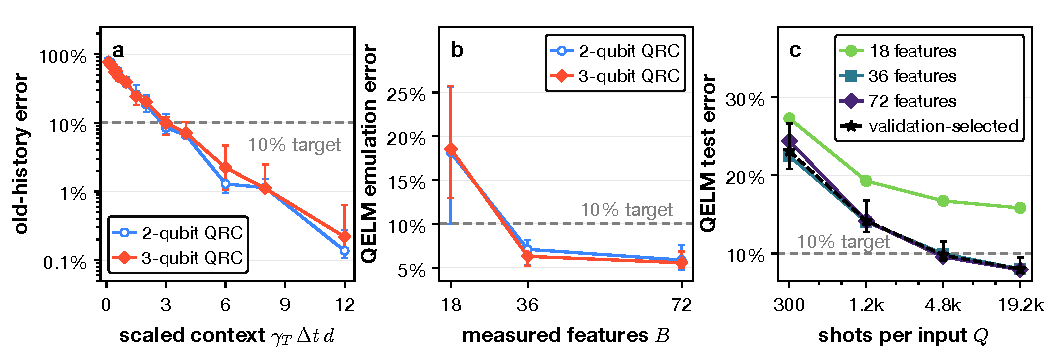
\includegraphics[width=\textwidth]{fig03_resource_diagnosis.pdf}
 \caption{\textbf{Three resources target three different limits.}
 \textbf{a} Longer windows reduce history NRMSE; curves are teacher-family
 medians and bands span the 10th--90th percentiles across roots.  \textbf{b}
 On the $\gamma_T=4,d=6$ slice, more measured features reduce total QELM
 NRMSE; faint curves are individual roots and heavy curves are teacher-family
 medians.  \textbf{c} More shots reduce total test NRMSE under finite
 measurement; curves are medians across 12 roots and the shaded selected-policy
 band spans their 10th--90th percentiles.  Dashed lines mark the NRMSE tolerance
 $0.10$.  \textbf{c} is a post-confirmatory four-qubit study with 16
 complete fit-and-selection replicates per root.}
 \label{fig:resource-diagnosis}
\end{figure*}
